% !TEX root =  ../MAIN.tex
\clearpage
\section{Data-driven Mutation Analysis: DAMAt}

\renewcommand{\APPR}{\textit{DAMAt}\xspace}

\subsection{Overview}

We address the following research questions:

%    \item RQ1 Is data-driven mutation cost affordable within the space context? This research question aims to determine if data-driven mutation testing is feasible in terms of costs related to the set-up of the system.
%    What to measure? Size of fault models. Lines of code added to inject probes.
%
%    %% oscar notes:
%    % - the first question is, we need a definition of feasible in terms of cost related to the setup of the system
%    %   - what is the baseline?
%    %   - how do we measure the cost of setting up data-driven (implementation complexity)?
%    %.    - human cost of setting up the fault model?
%    %     - size of the SUT in memory?
%    %     - SUT execution time per introduced fault, which is the fastest? \cite{winter2011impact}
%    %.      - given that a system may behave differently depending on the effect of the fault, the faults could be classified as no effect, test failure, application hang
%    %     - LoC (SLoCCount)
%    %     - cyclomatic complexity (SourceMonitor)?
%    % - injecting defects in every location of complex software leads to a dramatic increase of the cost of the campaign \cite{natella2012fault}
%
%    %  - fault latency: addresses the duration of an injection in terms of repeated fault activation. Transient faults are activated exactly once, intermittent faults are activated a finite number of times, and permanent faults are activated every time.
%    % - injection trigger: when the probe is activated \cite{winter2011impact}
%
%    \item RQ2 Does data-driven mutation scale in space context? Given the large quantity of data exchanged by space software components, there is a risk that data-driven mutation require the execution of a large number of test cases. This research question aims to determine if data-driven mutation testing can scale up.
%
%    \item RQ3 How does data-driven mutation compare to code-driven mutation in terms of effectiveness and test execution time? This research question aims to compare the results obtained with code-driven and data-driven test suite assessment. We are interested in answering the following subquestions:
%    \begin{itemize}
%    \item (RQ3.a) Do test cases that kill code-driven mutants tend kill also data-driven mutants?
%
%    %For each data-driven mutant we remove all the test cases (or, better, the oracles) that kill the mutant, then we verify if the code-driven mutation score changes. If the code-driven mutation score does not change it means that data-driven is complementary.
%
%    %For each code-driven mutant we remove all the test cases that kill the mutant, then we verify if the data-driven mutation score changes
%
%    %We shall consider only  code-driven mutants affecting the functionalities affected  by data-driven mutation.
%
%    \item (RQ3.b) What type of mutants generated by data-driven mutation are not detected by means of code-driven mutants?
%
%    %We keep a minimal set of test cases to kill all the data driven mutants
%    %We look for test cases that if removed do not change the code-driven mutation score
%    %If such test cases exists, it means that the data driven mutant that they kill, cannot be replaced through a code-driven mutant
%
%    \item  (RQ3.c) Is it possible to find a relation between the mutation scored computed with data-driven and code-driven mutation?
%    Measurements. Simple solution: (1) collect mutation score for code-driven and data-driven for all the subjects (2)  compute some correlation coefficient. Problem: too few subjects, not sure if correlation coefficient works with 3 subjects only. What does literature says on this matter?
%
%    \item (RQ3.d) Is data-driven mutation better than code-driven mutation in detecting test suites not capable of identifying problems in the implementation of requirements?
%
%    We assume that data-driven simulates fault in the implementation of requirements. Is it really the case?
%    Does it improve over code-driven?
%
%    To this end we inject faults in the software (e.g., faults manually derived after modifying the requirements) and compare how well data-driven/code-driven discover them.
%
%    We identify test suites with mutation score of 70\%, 60\%, 50\%
%    or we identify test suites achieving >90\% of the subject mutation score, >80\%, >70\%..
%    With "identify" I mean we select a subset of test cases  in the original test suite, to achieve the desired mutation score.
%    We compute the percentage of faults detected by the test cases killing at least one data-driven mutant.
%    We compute the percentage of faults detected by the test cases killing at least one code-driven mutant.
%    \end{itemize}
%
%
%    \item RQ4 To what extent equivalent and redundant mutants affect data-driven mutation? We aim to investigate how likely data-driven mutants are affected by the presence of equivalent and redundant mutants.
%
%    \item RQ5 Does mutants sampling lead to accurate results in the case of data-driven mutation testing? This re- search question investigates if mutants sampling is accurate also in the case of data-driven mutation testing.
%
%
%    \item RQ6 How do mutants sampling approaches compare in terms of performance? We aim to determine which mutants sampling strategy reduces most the data-driven mutation testing execution time.
%


\emph{RQ1. What are the types of test suite shortcomings identified by \APPR?}
    We aim to assess the effectiveness of \APPR in identifying various test suite shortcomings.  In other words, we want to know if mutation analysis based on \APPR can provide clear guidance in terms of what to improve in a test suite.
   % Further, we will discuss with engineers the reasons why mutants are not killed by the test suite and categorize  such shortcomings, e.g., lack of oracles verifying warning messages.
    %This research question aims to determine the test suite weaknesses by identifying the shortcomings of the test suites (e.g., lack of oracles).
    % This research questions aims to identify the type of faults that are harder to kill among CPSs test suites.

%FABRIZIO: the following has been removed for space reasons...
%\emph{RQ2. How are killed and live mutants distributed among mutation operators?}
%We study the distribution of killed mutants across mutation operators to determine if it is feasible to identify a subset of operators that is more effective than others in detecting test suite shortcomings.





\emph{RQ2.
What is the impact of equivalent and redundant data-driven mutants on the mutation analysis process?}
    In general, mutation analysis may lead to the generation of equivalent and redundant mutants.
    In the specific context of \APPR, we analyze the extent of their impact on mutation scores.
    %by re-calculating the mutation execution time and mutation score when removing such mutants from the analysis.}

\emph{RQ3.  Is data-driven mutation feasible?}
    To assess its feasibility in practice, we evaluate the cost of setting up data-driven mutation analysis (i.e., defining fault models and instrumenting the CPS with probes), {the duration of the mutation analysis process, and the} runtime overhead introduced during test case execution.


%\REVOCT{C-P-13}{Instead, we keep the following research questions for the FAQAS follow-on activity:}
%
%    \REVOCT{C-P-13}{\emph{RQ4. How does data-driven mutation compare to code-driven mutation?} This research question aims to compare the results obtained with code-driven and data-driven test suite assessment. We are interested in answering the following subquestions: (RQ4.a) Do test cases that kill code-driven mutants tend kill also data-driven mutants? (RQ4.b) What type of mutants generated by data-driven mutation are not detected by means of code-driven mutants? (RQ4.c) Is it possible to find a relation between the mutation scored computed with data-driven and code-driven mutation?}
%
%    \REVOCT{C-P-13}{\emph{RQ5. Does mutants sampling lead to accurate results in the case of data-driven mutation testing?} This research question investigates if mutants sampling is accurate also in the case of data-driven mutation testing.}
%
%    \REVOCT{C-P-13}{\emph{RQ6. How do mutants sampling approaches compare in terms of performance?} We aim to determine which mutants sampling strategy reduces most the data-driven mutation testing execution time.}
%
%    \REVOCT{C-P-13}{\emph{RQ7. Is it feasible to apply reachability analysis to automatically generate inputs that kill data-driven mutants?} This research question aims to evaluate, on a subset of the case study systems, if static analysis is a viable solution to generating test cases that kill data-driven mutants. We aim to address the following subquestions: (RQ7.a) Can static analysis generate inputs that trigger the mutants? (RQ7.b) Are the generated inputs valid (i.e., do they lead to valid executions or are discarded by the software)?}


\subsection{Subjects of the study}

%% !TEX root =  ../MAIN-DataDrivenMutationAnalysis.tex

\begin{table}[tb]
\caption{Descriptions of subject artifacts.}
\label{table:caseStudies} 
\footnotesize
\centering
\begin{tabular}{|
@{\hspace{1pt}}p{15mm}
@{\hspace{2pt}}|
@{\hspace{1pt}}>{\raggedleft\arraybackslash}p{10mm}@{\hspace{1pt}}|
@{\hspace{1pt}}>{\raggedleft\arraybackslash}p{20mm}@{\hspace{1pt}}|
@{\hspace{1pt}}>{\raggedleft\arraybackslash}p{18mm}@{\hspace{1pt}}|
p{20mm}|}
\hline
\textbf{Subject}&\textbf{LOC}&\textbf{Test suite type}&\textbf{\# Test cases}\\
\hline
\ESAIL & 74,155 & \multirow{5}{*}{System}& \multirow{5}{*}{384} \\
\SVF& 65,764 & &  \\
\ADCS& \multirow{3}{*}{NA} & &  \\
\GPS&  & &  \\
\PDHU&  & &  \\
%ESAIL execution time: 8.3 hours
\hline
\PARAM{}& 3,179 & Integration& 170 \\
%LIBPARAM execution time: 50 seconds
\hline
\end{tabular}

\end{table}


%To assess our research questions, we considered five software artifacts, developed by two of our industry partners for different satellites:  Attitude Determination And Control System (\ADCS), \GPS, Payload Data Handling Unit (\PDHU), the three subsystems developed by \LuxSpace for the \ESAIL satellite, and the Parameter system (\PARAM), CSP networking (\CSP) libraries developed by \GomSpace.

To assess our research questions, we consider \PARAM, which is a client-server component to manage configuration parameters in cubesats. \REVFINAL{A11}{Also, we consider \GCSP, which is component to manage networking communication on cubesats.}
Finally, we examine three \ESAIL software sub-systems (1) the Attitude Determination And Control System (\ADCS), the Global Positioning System (\GPS), and the Payload Data Handling Unit (\PDHU). {These are representative examples of control and utility software, as well as sensor and actuator drivers.}
%Detailed information about the fault models is provided in Appendix~\ref{appendix:FMS}. Additional experiments considering also LIBGCSP will be performed in WP4.

We rely on \APPR to evaluate the \PARAM integration test suite by  mutating the data exchanged between the client and server components of \PARAM.
\REVFINAL{A11}{For \GCSP, we mutate the data sent by a client application on the network.}
Finally, \APPR is used to evaluate how well the
\ESAIL test suite covers interoperability problems affecting the integration between the control software of \ESAIL (hereafter, CSW) and the \ADCS, \PDHU, and \GPS components. We thus
mutate the data exchanged between \ESAIL CSW and these three components.
Since each of these sub-systems have a  different purpose (i.e., their data is processed by distinct CSW functions and affect distinct \ESAIL features) we treat them as distinct case study subjects although they are tested using the same test suite. We focus on the \ESAIL test suite that makes use of an SVF to simulate the \ADCS, \PDHU, and \GPS components.
The main reason is that these three components can only be executed on the target hardware and thus most of the scenarios involving them are tested in a simulated environment first.
We do not mutate messages or data items that are tested only with HIL.

In the case of \PARAM, we inject mutation probes into the \PARAM server to mutate both received and generated messages. For \ESAIL, we insert mutation probes into the SVF that mutate the messages it generates; we avoid mutating the messages received by the SVF because such mutations may lead to input data it does not support.
%Table~\ref{table:summary} provides further information about our case study subjects.
\ESAIL features 74 kLoC and its SVF 65 kLoC.
The \ESAIL test suite includes 384 test cases, takes approximately 10 hours to execute, and relies on three simulated
\SVF sub-systems (i.e., \ADCS, \GPS, and \PDHU).
Instead, \PARAM contains 3 kLoC and is tested through an integration test suite which is composed by 170 test cases.
The \PARAM integration test suite takes approximately 1 minute to execute.
By considering both a quick integration test suite and an extensive system test suite, we aim to cover the diversity of scenarios in which our approach can be applied.


%\GomSpace subject is compiled with the Gnu Compiler Collection (GCC) for Linux x86 version 6.3.
%Instead, \LuxSpace subjects rely on Clang++ Compiler for Linux x86\_64 version 5.0.0.


\subsection{Experimental Setup}


With the support of our industry partners, we relied on
 the systems' specification documents
 %(i.e., the Interface Control Document and the Software User Manual, based on the ECSS standard)
 to define the fault models for each subject.


%Note that we did not target every data item being exchanged between components, since input partitions for certain data items (e.g., nominal and non-nominal cases) are covered only by test suites with hardware in-the-loop.

% we based on the specifications of the systems, provided the type of ECSS document, and selected only operators that cover a fault that shall be discovered by the test suite

% (i.e., the rest of faults are covered by test suites with hardware in-the-loop).
%We used this information as an input for \APPR and consequently applied the six steps of the approach.

% !TEX root =  ../MAIN-DataDrivenMutationAnalysis.tex

\begin{table}[tb]
\caption{Fault models and mutation operators.}
\label{table:summary} 
\center
\footnotesize
\begin{tabular}{|
@{\hspace{1pt}}p{24mm}@{\hspace{0pt}}|
@{\hspace{0pt}}>{\raggedleft\arraybackslash}p{17mm}@{\hspace{1pt}}|
@{\hspace{0pt}}>{\raggedleft\arraybackslash}p{25mm}@{\hspace{1pt}}|
@{\hspace{0pt}}>{\raggedleft\arraybackslash}p{25mm}@{\hspace{1pt}}|
p{4mm}|}
\hline
\textbf{Subject}&\textbf{Fault Models}&\textbf{Configured Operators}&\textbf{Mutation Operations}\\
\hline
\ADCS& 10 & 142 & 172 \\
\GPS& 1 & 23 & 23 \\
\PDHU& 3 & 29 & 29 \\
\PARAM& 6 & 80 & 80 \\
\hline
\end{tabular}
\end{table}



{Table~\ref{table:summary} provides information about the fault models.}
The fault models (FMs) for the \ADCS include multiple configurations (\INDEX{Configured operators}) of eight mutation operators: BF, VAT, VBT, VOR, IV, FVOR, FVBT, and FVAT.
The \PDHU fault models include four operators: BF, IV, VAT and FVAT.
Even though the \GPS fault model concerns only one data type, it makes use of six operators: ASA, HV, IV, SS, VAT, and FVAT.
For \PARAM, we relied on the operators BF, HV, IV, SS, VAT, and FVAT.
\REVFINAL{A11}{For \GCSP, we relied on the operators INV, VAT, FVAT, BF, VOR, FVOR, and SS.}
All the mutation operators provided by \APPR have been used in at least one fault model, which shows their usefulness.
{They have led to 172 mutation operations for \ADCS, 23 for \GPS, 29 for \PDHU, 44 for \PARAM, and 33 for \GCSP; the number of configured operators and mutation operations match except when we rely on VOR and FVOR.}

%Table~\ref{table:summary} provides information about the different fault models that were specified, which consist of 119 mutation operations for \ADCS, 26 for \GPS, 59 for \PDHU, and 35 for  \PARAM.
%, and \TODO{ZZ} for the \CSP.
%After considering all the mutation operators specified in Table~\ref{table:operators_DDMA}, for \ADCS, this led to five mutation operators: BF, VAT, VBT, VOR, and IV.
%Similarly, in the case of \PDHU,
%we considered four mutation operators: BF, IV, VAT and FVAT.
%Even though the \GPS fault model concerns only one data type, it makes use of five mutation operators: ASA, HV, IV, SS, and VAT.
%For \PARAM, we made use of the mutation operators BF, HV, IV, SS, and VAT.
%Since all the mutation operators have been used in at least one fault model, we can consider all of them to be useful.

%In general, our subjects include \TODO{the same} ratio of operators per fault model specification,%type,
 %thus showing that all operators are useful.

We performed our experiments using an HPC cluster with Intel Xeon E5-2680 v4 (2.4 GHz) nodes.

%To perform our empirical evaluation,
%We implemented \APPR in a toolset that is available under the ESA Software Community Licence Permissive, at the following URL \textbf{https://blind/}.


\subsection{RQ1 - Approach effectiveness}
\label{sec:empirical:damat:rq1}

% \subsubsection*{Design and measurements}

We analyzed the extent to which \APPR helps identify limitations in test suites.
For each subject, we inspected uncovered fault models, uncovered mutation operations, and live mutants. We then analyzed how they could potentially be explained by the types of possible shortcomings:
untested message types (UMT), \REVOCT{C-P-14}{uncovered input partitions\footnote{An input partition is a set of values or value ranges; such sets partition the input domain into regions with values that are equivalent from a testing viewpoint. Input space partitioning is a traditional functional testing approach~\cite{ammann2016introduction}. In \APPR, each mutation operation covers (i.e., alters) values belonging to a specific input partition; therefore, the lack of coverage of a mutation operation indicates that an input partition was not tested.}} (UIP), poor oracle quality (POQ), and lack of test inputs (LTI).
To achieve the above, we proceeded as follows.
For each uncovered fault model, we discussed with developers if the functionality triggering the exchange of the targeted message was tested by the test suite.
For uncovered mutation operations, we discussed with engineers if they match an uncovered input partition.
For live mutants, we determined if they could be killed by improving test oracles (see how equivalent mutants are detected for RQ2).
%(e.g., lack of oracles concerning internal state variables, lack of inputs triggering exceptional scenarios).

To address RQ1, based on the above analysis, we discuss below how our metrics (i.e., \INDEX{fault model coverage - FMC}, \INDEX{mutation operation coverage - MOC}, and \INDEX{mutation score - MS}) relate to the predefined shortcoming categories {(e.g., a low mutation score may indicate missing test oracles)}.
%For example, a low mutation score may indicate missing test oracles, or a low fault model coverage level may suggest a lack of test cases for certain functionalities.
\CHANGED{Further, to understand how variations in test effectiveness could be explained, we investigate how our metrics relate to the number of functionalities under test (i.e., the number of fault models - $\mathit{FM}$), the number of mutation operations ($MO$), and the number of covered mutation operations ($CMO$), respectively.
To get an idea of observable trends, we compute the Spearman's correlation coefficients between them, hereafter denoted $\rho_{FM}$, $\rho_{MO}$, $\rho_{CMO}$.}

%Concerning UIP and POQ we distinguish between nominal and non-nominal scenarios.
%\emph{UIP for non-nominal (nominal) scenarios} indicate that the test suite triggers the exchange of data items targeted in the fault model but it does not exercise the non-nominal (nominal) cases. For example, the test suite may cause the retrieval of the board voltage only in the case of voltage within range.
%\emph{POQ for non-nominal (nominal) scenarios} indicate that the test suite triggers the exchange of data item instances that are representative for the non-nominal (nominal) case (e.g., error messages are exchanged by components) however the oracles do not appropriately verify outputs. For example, the test suite may not verify if error messages had been actually exchanged.



%Furthermore, for each subject, we report the mutation analysis results in terms of the metrics defined in Section~\ref{sec:mutantsExecution}: \emph{fault model coverage}, \emph{mutation operation coverage}, and \emph{mutation score}.



%A description of the possible shortcomings that can be identified by \APPR follows.
%The possible shortcomings that can be identified by \APPR had been introduced in Section~\ref{}:
%untested message types (UMT), uncovered input partitions (UIP), poor oracle quality (POQ), and lack of test inputs (LTI).
%To better characterize our results we have refined UMT, UIP, and POQ into subclasses that are reported in the following.
%
%\emph{UMT - Functionality not tested:} the test suite does not exercise the exchange of the messages targeted by the given fault model because engineers mistakenly forget to test one functionality.
%%This type of shortcoming can be reflected on the \emph{fault model coverage} metric.
%
%%\emph{Lack of input partitions for a functionality} means the test suite includes a testing scenario, but it does not include configurations for a component related to the targeted data item.
%
%\emph{UIP - Lack of simulations for nominal scenarios:} the test suite triggers the exchange of the targeted data items but it does not exercise the nominal case (e.g., it tests the retrieval of the board voltage only in the case of voltage out of range).
%\emph{UNIP - Lack of simulations for non-nominal scenarios:} the test suite triggers the exchange of the targeted data items but it does not exercise the nominal case (e.g., it tests the retrieval of the board voltage only in the case of voltage within range).
%
%%Lack of simulated configurations and input partitions are reflected on the \emph{mutation operation coverage} metric.
%
%\emph{Lack of oracles concerning log-files from hardware} means that the test suite covers a testing scenario for the targeted data item, and includes test cases for a specific input partition, but it does not verify possible warnings coming from hardware components.
%\emph{Lack of oracles for return codes} means that the test suite covers the testing scenario and input partition, but it does not verify the return codes coming from a certain component.
%\emph{Lack of oracles concerning non-nominal scenarios} means that the test suite covers the exceptional testing scenarios and input partitions, but it does not verify if warnings are produced, but simply check that redundancy mechanisms work.
%\emph{Lack of oracles concerning internal state variables} means the test suite covers a testing scenario and a specific input partition, but it does not verify internal or intermediate state variables.
%Lack of oracles reflects directly on the \emph{mutation score} metric.


\subsubsection*{Results}

% !TEX root =  ../MAIN-DataDrivenMutationAnalysis.tex

\begin{table}[tb]
\caption{Mutation Analysis Results.}
\label{table:mutationresults} 
\center
\footnotesize
\begin{tabular}{|
@{\hspace{0pt}}>{\raggedleft\arraybackslash}p{24mm}@{\hspace{1pt}}|
@{\hspace{0pt}}>{\raggedleft\arraybackslash}p{12mm}@{\hspace{1pt}}|
@{\hspace{0pt}}>{\raggedleft\arraybackslash}p{12mm}@{\hspace{1pt}}|
@{\hspace{0pt}}>{\raggedleft\arraybackslash}p{13mm}@{\hspace{1pt}}|
@{\hspace{0pt}}>{\raggedleft\arraybackslash}p{12mm}@{\hspace{1pt}}|
@{\hspace{0pt}}>{\raggedleft\arraybackslash}p{12mm}@{\hspace{1pt}}|
@{\hspace{0pt}}>{\raggedleft\arraybackslash}p{12mm}@{\hspace{1pt}}|
@{\hspace{0pt}}>{\raggedleft\arraybackslash}p{12mm}@{\hspace{1pt}}|
@{\hspace{0pt}}>{\raggedleft\arraybackslash}p{12mm}@{\hspace{1pt}}|
}
\hline
\textbf{Subject} & 
\textbf{\# FMs} & 
\textbf{FMC} & 
\textbf{\#MOs-CFM} & 
\textbf{\#CMOs} & 
\textbf{MOC}  
&\textbf{Killed}&\textbf{Live}&\textbf{MS}
\\
\hline

\ADCS &10 &90.00\%   & 135 & 100 & 74.00\%   &    45&55&45.00\%\\
\GPS &1 &100.00\%    &  23  &  22 & 95.65\%    &      21&1&95.45\%\\
\PDHU &3 &100.00\%  &   29 & 24 & 82.76\%   &     24&0&100.00\%\\
\PARAM &6 &100.00\%  &   44 & 41 & 93.20\%  &        37&4&90.24\%\\
\GCSP &1 &100.00\%  &   33 & 21 & 63.64\%  &        NA&NA&NA\\


\hline

\end{tabular}

CMO=Covered Mutation Operation, MOs-CFM=Mutation Operations in covered FMs.

\end{table}


% !TEX root =  ../MAIN-DataDrivenMutationAnalysis.tex


\begin{table}[tb]
\caption{Shortcomings of CPSs test suites.}
\label{table:shortcomings} 
\center
\footnotesize
\begin{tabular}{|
@{\hspace{1pt}}p{10mm}
@{\hspace{1pt}}|
@{\hspace{2pt}}>{\raggedleft\arraybackslash}p{5mm}@{\hspace{4pt}}|
@{\hspace{2pt}}>{\raggedleft\arraybackslash}p{5mm}@{\hspace{4pt}}|
@{\hspace{-1pt}}>{\raggedleft\arraybackslash}p{5mm}@{\hspace{2pt}}|
>{\raggedleft\arraybackslash}p{5mm}@{\hspace{4pt}}|
@{\hspace{2pt}}>{\raggedleft\arraybackslash}p{5mm}@{\hspace{4pt}}|
@{\hspace{-1pt}}>{\raggedleft\arraybackslash}p{5mm}@{\hspace{2pt}}|
>{\raggedleft\arraybackslash}p{5mm}@{\hspace{4pt}}|
@{\hspace{2pt}}>{\raggedleft\arraybackslash}p{5mm}@{\hspace{4pt}}|
@{\hspace{-1pt}}>{\raggedleft\arraybackslash}p{5mm}@{\hspace{2pt}}|
>{\raggedleft\arraybackslash}p{5mm}@{\hspace{4pt}}|
@{\hspace{2pt}}>{\raggedleft\arraybackslash}p{5mm}@{\hspace{4pt}}|
@{\hspace{-1pt}}>{\raggedleft\arraybackslash}p{5mm}@{\hspace{2pt}}|
p{2mm}|
@{\hspace{2pt}}>{\raggedleft\arraybackslash}p{5mm}@{\hspace{4pt}}|
@{\hspace{-1pt}}>{\raggedleft\arraybackslash}p{5mm}@{\hspace{2pt}}|
p{2mm}|}
\hline
\textbf{Short-}      & \multicolumn{3}{c|}{\textbf{\ADCS}} & \multicolumn{3}{c|}{\textbf{\GPS}} & \multicolumn{3}{c|}{\textbf{\PDHU}} & \multicolumn{3}{c|}{\textbf{\PARAM}}& \multicolumn{3}{c|}{\textbf{\GCSP}} \\
\textbf{coming} & \textbf{UF}&\textbf{UM} &\textbf{LM} & \textbf{UF}&\textbf{UM} &\textbf{LM} & \textbf{UF}&\textbf{UM} &\textbf{LM} & \textbf{UF}&\textbf{UM} &\textbf{LM}
& \textbf{UF}&\textbf{UM} &\textbf{LM}\\
\hline 
UMT                              &1&-&-&-&-&-&-&-&-&-&-&-&-&-&-\\
% Lack of input partitions for a functionality  & & & & & & & & & & & & \\
UIP     &-&35&-&-&1&-&-&5&-&-&7&-&-&12&-\\
POQ         &-&-&55&-&-&1&-&-&-&-&-&4&-&-&-\\
LTI         &-&-&-&-&-&-&-&-&-&-&-&-&-&-&-\\
\hline
\textbf{Total} &1&35&55&-&1&1&-&5&-&-&7&4&-&12&-\\
\hline
\end{tabular}

UF=Uncovered Fault model, UM=Uncovered Mutation operation, LM=Live mutant.
\end{table}





%\begin{table*}[tb]
%\caption{Shortcomings of CPSs test suites.}
%\label{table:shortcomings} 
%\footnotesize
%\centering
%\begin{tabular}{|
%@{\hspace{1pt}}p{60mm}
%@{\hspace{1pt}}|
%@{\hspace{2pt}}>{\raggedleft\arraybackslash}p{7mm}@{\hspace{4pt}}|
%@{\hspace{2pt}}>{\raggedleft\arraybackslash}p{7mm}@{\hspace{4pt}}|
%@{\hspace{-1pt}}>{\raggedleft\arraybackslash}p{6mm}@{\hspace{2pt}}|
%>{\raggedleft\arraybackslash}p{7mm}@{\hspace{4pt}}|
%@{\hspace{2pt}}>{\raggedleft\arraybackslash}p{7mm}@{\hspace{4pt}}|
%@{\hspace{-1pt}}>{\raggedleft\arraybackslash}p{6mm}@{\hspace{2pt}}|
%>{\raggedleft\arraybackslash}p{7mm}@{\hspace{4pt}}|
%@{\hspace{2pt}}>{\raggedleft\arraybackslash}p{7mm}@{\hspace{4pt}}|
%@{\hspace{-1pt}}>{\raggedleft\arraybackslash}p{6mm}@{\hspace{2pt}}|
%>{\raggedleft\arraybackslash}p{7mm}@{\hspace{4pt}}|
%@{\hspace{2pt}}>{\raggedleft\arraybackslash}p{7mm}@{\hspace{4pt}}|
%@{\hspace{-1pt}}>{\raggedleft\arraybackslash}p{6mm}@{\hspace{2pt}}|
%p{2mm}|}
%\hline
%     & \multicolumn{3}{c|}{\textbf{\ADCS}} & \multicolumn{3}{c|}{\textbf{\GPS}} & \multicolumn{3}{c|}{\textbf{\PDHU}} & \multicolumn{3}{c|}{\textbf{\PARAM}} \\
%\hline
%\textbf{Test suite shortcoming} & \multicolumn{3}{c|}{\textbf{\#Mutants}}& \multicolumn{3}{c|}{\textbf{\#Mutants}} &\multicolumn{3}{c|}{\textbf{\#Mutants}} &\multicolumn{3}{c|}{\textbf{\#Mutants}}          \\
% & \textbf{FMNC}&\textbf{MONC} &\textbf{LM} & \textbf{FMNC}&\textbf{MONC} &\textbf{LM} & \textbf{FMNC}&\textbf{MONC} &\textbf{LM} & \textbf{FMNC}&\textbf{MONC} &\textbf{LM}\\
%\hline 
%A functionality is not tested                              &37&-&-&-&-&-&-&-&-&-&-&-\\
%% Lack of input partitions for a functionality  & & & & & & & & & & & & \\
%Lack of simulated configurations for nominal scenarios     &-&7&-&-&-&-&-&-&-&-&1&-\\
%Lack of simulated configurations for non-nominal scenarios &-&37&-&-&1&-&-&5&-&-&7&-\\
%Lack of oracles concerning log-files from hardware         &-&-&30&-&-&1&-&-&-&-&-&-\\
%Lack of oracles for return codes                           &-&-&18&-&-&-&-&-&-&-&-&-\\
%Lack of oracles concerning non-nominal scenarios           &-&-&2&-&-&-&-&-&-&-&-&-\\
%Lack of oracles concerning internal state variables        &-&-&1&-&-&-&-&-&-&-&-&43\\
%\hline
%\textbf{Total} &37&44&51&-&1&1&-&5&-&-&8&43\\
%\hline
%\end{tabular}
%
%\textbf{Legend:} FMNC=Fault model not covered, MONC=Mutation operation not covered, LM=Live mutant.
%\end{table*}

Table~\ref{table:mutationresults} reports the mutation analysis results according to our metrics.
In Table~\ref{table:shortcomings}, we report how uncovered fault models, uncovered mutation operations, and live mutants are distributed with respect to the different shortcomings we noticed on each subject.

\REVFINAL{A11}{Concerning \INDEX{fault model coverage}, \ADCS reached a coverage of 90.00\%, while \GPS, \PDHU, \PARAM, and \GCSP all achieved 100\%.}
%$\rho_{FM}$ = -0.90,
%$\rho_{FM}$ = -0.77,
%we see that,
As expected, the much higher number of messages to test for \ADCS leads to incomplete testing.

\ADCS reached 74\% \INDEX{mutation operation coverage}. \REVFINAL{A11}{\GCSP achieved 63.64\%.} \GPS, \PDHU, and \PARAM  achieved even higher coverage with 95.65\%, 82.76\%, and 93.20\%,  respectively. Since
%$\rho_{FM}$ = -0.97 and $\rho_{MO}$ = -0.98,
%$\rho_{FM}$ = -1 and
$\rho_{MO}$ = -0.5, results suggest that lower mutation operation coverage is more likely when systems are more complex (i.e., there are many mutation operations, whose numbers depend on the number of input partitions).

Regarding \INDEX{mutation scores}, we report 45.00\% for \ADCS,  95.45\% for \GPS,  and 100.00\% for \PDHU. These results indicate a varying performance of the \SVF test suite across sub-systems.
\REVFINAL{A11}{\PARAM obtained a mutation score of 90.24\%.
For \GCSP, we could not compute the mutation score because after mutation, the test suite has shown non-deterministic outcomes probably due to delays introduce by the mutation itself --- \GCSP is tested with stringent time requirements.}
% indicating that only slightly more than a third of mutants are killed by the test suite.
Given that
%$\rho_{FM}$ = -0.80, $\rho_{MO}$ = -0.80, and $\rho_{CMO}$ = -0.86,
%$\rho_{FM}$ = -0.6, $\rho_{MO}$ = -0.6, and
$\rho_{CMO}$ = -0.6,
we conclude that the mutation score tends to be lower for complex systems with a large number of covered mutation operations.
%Different from the other metrics,  mutation scores do not appear dependent on the size of the fault model.

Table~\ref{table:shortcomings} provides the shortcomings identified for all our subjects.
Our analysis confirms that (1) uncovered fault models (i.e., low \INDEX{FMC}) indicate lack of coverage for certain message types (\INDEX{UMT}) and, in turn, the lack of coverage of a specific functionality (i.e., setting the pulse-width modulation in \ADCS); (2) uncovered mutation operations (i.e., low \INDEX{MOC}) highlight the lack of testing of input partitions (\INDEX{UIP}); (3) live mutants (i.e., low \INDEX{MS}) suggest poor oracle quality (\INDEX{POQ}). In our case study systems the presence of live mutants was not explained by the lack of test inputs in the original test suite. Moreover, we have not uncovered latent faults, which is unsurprising given that all these systems went through all testing stages, including HIL, and are on orbit.

%\subsection{RQ2 - Operators effectiveness}
%
%% \subsubsection*{Design and measurements}
%%RQ2 aims to investigate differences in results across \APPR operators.
%A mutation operator is effective if it leads to mutants that enable detecting uncovered input partitions, poor oracle quality, or lack of test inputs. For each subject, we thus report the proportion of mutation operators that lead to such cases (i.e., mutants that are hard to kill).
%In general, hard to kill mutants indicate to practitioners how to prioritize the execution of mutants during the data-driven mutation analysis process (hard to kill mutants shall be executed first).
%
%
%
%We identify the type of faults that are harder to kill by analyzing the mutation scores across operators.%distribution of killed mutants across operators.
%In general, faults that are harder to kill may indicate to practitioners which fault types to prioritize during the data-driven mutation analysis process.%, since they may hide subtle problems of the test suite.
%
%%We measure the proportion of shortcomings detected by prioritizing the execution of operators.
%
%% For each subject, we report the coverage metrics defined in  Section~\ref{sec:mutantsExecution}: \emph{fault model coverage},  \emph{mutation operation coverage}, and \emph{mutation score}.
%
%\subsubsection*{Results}
%
%%Operators that are killed most are the ones that concern data provided by sensors, which is often the one verified by test cases.
%%The operator that is less killed is the BF, which is used for configuration options or state information that is usually not verified by the oracles.
%%
%%
%%
%%\TODO{TBD}
%
%% !TEX root =  ../MAIN-DataDrivenMutationAnalysis.tex

\begin{table}[tb]
\caption{Mutation operators effectiveness.}
\label{table:killed_fault_classes} 
\scriptsize
\centering
\begin{tabular}{|
@{\hspace{1pt}}p{10mm}
@{\hspace{2pt}}|
@{\hspace{1pt}}>{\raggedleft\arraybackslash}p{17mm}@{\hspace{1pt}}|
@{\hspace{1pt}}>{\raggedleft\arraybackslash}p{17mm}@{\hspace{1pt}}|
@{\hspace{1pt}}>{\raggedleft\arraybackslash}p{17mm}@{\hspace{1pt}}|
@{\hspace{1pt}}>{\raggedleft\arraybackslash}p{16mm}@{\hspace{1pt}}|
p{20mm}|}
\hline
\textbf{Mutation operator}&\textbf{\ADCS operators effectiveness (\%)}&\textbf{\GPS\hspace{1mm} operators effectiveness (\%)}&\textbf{\PDHU operators effectiveness (\%)}&\textbf{\PARAM\hspace{2mm} operators effectiveness (\%)}\\
\hline
BF	 &80.00&&0.00&50.00\\
FVAT &100.00&100.00&100.00&100.00\\
IV	 &100.00&0.00&14.29&20.00\\
VOR	 &66.67&&&\\
VBT	 &100.00&&&\\
FVBT &100.00&&&\\
VAT	 &14.81&0.00&0.00&42.86\\
FVOR &55.56&&&\\
ASA  &&0.00&&\\
SS   &&11.11&&79.17\\
HV   &&0.00&&0.00\\
\hline
\end{tabular}

\end{table}

%
%Table~\ref{table:killed_fault_classes} presents the distribution of hard to kill mutants across the types of mutation operators implemented by \APPR. In general, it is not feasible to identify a subset of operators that is more effective than others; indeed all the operators show a varying proportion of hard to kill mutants across subjects. Such result may be due to our set of operators being representative and reduced.
%



\subsection{RQ2 - Equivalent and redundant mutants}
\label{sec:rq2:damat}

% \subsubsection*{Design and measurements}

As they potentially have significant impact on the applicability of any mutation analysis approach, we assess the impact of equivalent and redundant mutants generated by \APPR.
%Equivalent and redundant mutants inflate the mutation score and thus prevent the correct assessment of the test suite. This question aims to determine whether this is a significant problem with \APPR.

%Equivalent mutants are modified versions of the SUT that have the same visible output as the original SUT.
%Instead, redundant mutants are modified versions of the SUT that have the same visible output as other mutants (e.g., two mutants causing the same failures in the test suite).

% consist of modified data (i.e., data altered by means of mutation operators) that do not lead to any noticeable difference in the output of the SUT with respect to the original version of the data.
%Instead, redundant mutants cause the same failures in the test suite.%, and consequently inflating the mutation score.%preventing the correct assessment of the test suite.
%Two are the reasons for redundant mutants. First,
%The reason for redundant mutants is that
%mutations alter different instances of a same data structure in the same way (e.g., delete a message in a sequence).

%Second, the mutations alter data chunks that are ignored by the oracles of the test suite.

%For every subject, we report the number of equivalent and redundant mutants.
We determined if a live mutant is nonequivalent by verifying, with the support of our industry partners,
if there existed a test case that, after performing the mutation operation, would generate one observable output (e.g., log entry, state variable, or data sent in response to test inputs) that differs from the one generated by the original program. Otherwise a mutant was considered equivalent.

According to related work, two mutants should be considered redundant if they produce the same observable output for every possible input~\cite{Shin:TSE:DCriterion:2018}.
%Recent research work has shown that two mutants shall be considered redundant only if it is not possible to identify inputs that distinguish them~\cite{Shin:TSE:DCriterion:2018}; in turn, two mutants are redundant when they produce the same observable output for every possible input.
Since, with large software systems, it is not possible to automatically determine if such condition holds (e.g., differential symbolic execution may not scale and is hardly applicable when components communicate through a network), we rely on manual inspection. To make such such analysis feasible, we first need to select a subset of mutant pairs that are likely to be redundant (e.g., mutants that produce the same output for every executed test case).
However, the size of the software systems under analysis prevents the collection of all the observable outputs produced by the system.
%(e.g., only the filtering of nondeterministic data such as timestamps requires a great deal of effort and domain knowledge); for this reason we focus on the data processed by assertions.
%Unfortunately, it is not feasible to simply collect the data processed by assertions because assertions often process aggregated results generated by test utility functions (e.g., to determine if loss of  communication between \ESAIL-CSW and \ADCS has been detected, reported, and recovered it is necessary to inspect log files for the presence of corresponding log entries in appropriate order).
We thus select as likely to be redundant all the pairs of killed mutants that (1) are exercised by the same test cases and (2) present the same failing assertions for every test case. We then manually inspect the test cases to determine if an additional assertion or a different test input might lead to different results for the two mutants. Similar to related work, we exclude live mutants from this analysis~\cite{papadakis2016threats}.

%Since, with large CPSs, it is not possible to automatically determine if such condition holds (e.g., differential symbolic execution is not applicable when components rely on floating point arithmetic or communicate through means different than method calls), we shall rely on manual inspection. To make such analysis feasible, we first need to select a subset of mutant pairs that are likely redundant, that is, mutant pairs that produce the same output for every executed test case.
%However, the size of the CPSs under analysis prevents the collection of all the observable outputs produced by the system (e.g., only the filtering of nondeterministic data such as timestamps requires a great deal of effort and domain knowledge); for this reason we focus on the data processed by assertions. Unfortunately, collecting the data processed by assertions is not straightforward because assertions often process aggregated results generated by test utility functions, e.g., to determine if loss of  communication between \ESAIL-CSW and \ADCS has been detected, reported, and recovered it is necessary to inspect log files for the presence of corresponding log entries in appropriate order.
%We thus select as likely redundant all the pairs of killed mutants that (1) are exercised by the same test cases and (2) present the same failing assertions for every test case. We then manually inspect the test cases to determine if an additional assertion or a different test input (e.g., different simulator configuration) may distinguish the two mutants. Similarly to related work, we exclude live mutants~\cite{papadakis2016threats}.




%% !TEX root =  ../MAIN-DataDrivenMutationAnalysis.tex

\begin{table}[tb]
\caption{Equivalent and Redundant Mutants.}
\label{table:eq_red} 
\scriptsize
\centering

\begin{tabular}{|
p{12mm}|
@{\hspace{1pt}}>{\raggedleft\arraybackslash}p{14mm}@{\hspace{1pt}}|
               >{\raggedleft\arraybackslash}p{13mm}@{\hspace{1pt}}|
 >{\raggedleft\arraybackslash}p{15mm}@{\hspace{1pt}}|
  >{\raggedleft\arraybackslash}p{13mm}@{\hspace{1pt}}|
}

\hline
\textbf{Subject} & \multicolumn{2}{c|}{\textbf{Equivalents}}  & \multicolumn{2}{c|}{\textbf{Redundants}}  \\
\textbf{}
&\textbf{\# live mutants}&\textbf{\# equivalents}
&\textbf{\# selected pairs}&\textbf{\# redundants}\\
\hline

\ADCS  &60&0&    55&0\\
\GPS   &1&0&      3&0\\
\PDHU  &0&0&     14&0\\
\PARAM &45&0&    13&0\\


\hline

\end{tabular}

\end{table}


%% !TEX root =  ../MAIN-DataDrivenMutationAnalysis.tex

\begin{table*}[tb]
\caption{Shortcomings of CPSs test suites.}
\label{table:shortcomings} 
\footnotesize
\centering
\begin{tabular}{|
@{\hspace{1pt}}p{60mm}
@{\hspace{1pt}}|
@{\hspace{2pt}}>{\raggedleft\arraybackslash}p{7mm}@{\hspace{4pt}}|
@{\hspace{2pt}}>{\raggedleft\arraybackslash}p{7mm}@{\hspace{4pt}}|
@{\hspace{-1pt}}>{\raggedleft\arraybackslash}p{6mm}@{\hspace{2pt}}|
>{\raggedleft\arraybackslash}p{7mm}@{\hspace{4pt}}|
@{\hspace{2pt}}>{\raggedleft\arraybackslash}p{7mm}@{\hspace{4pt}}|
@{\hspace{-1pt}}>{\raggedleft\arraybackslash}p{6mm}@{\hspace{2pt}}|
>{\raggedleft\arraybackslash}p{7mm}@{\hspace{4pt}}|
@{\hspace{2pt}}>{\raggedleft\arraybackslash}p{7mm}@{\hspace{4pt}}|
@{\hspace{-1pt}}>{\raggedleft\arraybackslash}p{6mm}@{\hspace{2pt}}|
>{\raggedleft\arraybackslash}p{7mm}@{\hspace{4pt}}|
@{\hspace{2pt}}>{\raggedleft\arraybackslash}p{7mm}@{\hspace{4pt}}|
@{\hspace{-1pt}}>{\raggedleft\arraybackslash}p{6mm}@{\hspace{2pt}}|
p{2mm}|}
\hline
     & \multicolumn{3}{c|}{\textbf{\ADCS}} & \multicolumn{3}{c|}{\textbf{\GPS}} & \multicolumn{3}{c|}{\textbf{\PDHU}} & \multicolumn{3}{c|}{\textbf{\PARAM}} \\
\hline
\textbf{Test suite shortcoming} & \multicolumn{3}{c|}{\textbf{\#Mutants}}& \multicolumn{3}{c|}{\textbf{\#Mutants}} &\multicolumn{3}{c|}{\textbf{\#Mutants}} &\multicolumn{3}{c|}{\textbf{\#Mutants}}          \\
 & \textbf{FMNC}&\textbf{MONC} &\textbf{LM} & \textbf{FMNC}&\textbf{MONC} &\textbf{LM} & \textbf{FMNC}&\textbf{MONC} &\textbf{LM} & \textbf{FMNC}&\textbf{MONC} &\textbf{LM}\\
\hline 
A functionality is not tested                              &37&-&-&-&-&-&-&-&-&-&-&-\\
% Lack of input partitions for a functionality  & & & & & & & & & & & & \\
Lack of simulated configurations for nominal scenarios     &-&7&-&-&-&-&-&-&-&-&-&-\\
Lack of simulated configurations for non-nominal scenarios &-&28&-&-&1&-&-&5&-&-&7&-\\
Lack of oracles concerning log-files from hardware         &-&-&39&-&-&1&-&-&-&-&-&-\\
Lack of oracles for return codes                           &-&-&18&-&-&-&-&-&-&-&-&-\\
Lack of oracles concerning non-nominal scenarios           &-&-&2&-&-&-&-&-&-&-&-&-\\
Lack of oracles concerning internal state variables        &-&-&1&-&-&-&-&-&-&-&-&45\\
\hline
\textbf{Total} &37&35&60&-&1&1&-&5&-&-&7&45\\
\hline
\end{tabular}

\textbf{Legend:} FMNC=Fault model not covered, MONC=Mutation operation not covered, LM=Live mutant.
\end{table*}

%Table~\ref{table:eq_red} provides the results.

\subsubsection*{Results.}
All live mutants (i.e., 55 mutants for \ADCS, 1 mutant for \GPS, and 4 mutants for \PARAM) generate outputs that differ from the original software system and, therefore, we did not detect any equivalent mutant. Though it needed to be confirmed, such result was expected since our methodology, if correctly applied, suggests, for every data item, a set of mutation operators that, by construction, should not lead to mutated data that is equivalent to the original data.
Live mutants can be killed by introducing oracles that (1) verify additional entries in the log files (39 instances for \ADCS, 1 instance for \GPS), (2) verify additional observable state variables (14 instances for \ADCS, 4 instances for \PARAM), and (3) verify not only the presence of error messages but also their content (2 instances for \ADCS).
\REVOCT{C-P-18}{Such oracles may consist of additional assertions that verify data values already produced by the software under test (i.e., no modification of the SUT is needed).}


We did not find redundant mutants either, which was expected since (1) mutations concerning different data items, by definition, are expected to lead to different outputs, (2) the set of operators applied to a same data item, if selected according to our methodology, cannot lead to mutated data that is redundant.
All the pairs of likely redundant mutants were due to five situations: (1) the test case does not distinguish failures across data items (e.g., temperature values collected by different sensors),
(2) the test case does not distinguish errors across different messages (e.g., in \ADCS, the IfHK message reporting a broken sensor or the message sent by a sensor reporting malfunction), (3) the test case does not distinguish between errors in nominal and non-nominal data (e.g., it does not distinguish between VOR and FVOR), (4) the test case does not distinguish between upper and lower bounds (e.g., the mutants for VOR lead to the same assertion failures), and {(5) the test case does not distinguish between different error codes (i.e, it simply verifies that an error code is generated)}. Addressing such shortcomings make test cases more useful for root cause analysis.

\subsection{RQ3 - Feasibility}
\label{sec:rq3:damat}

% \subsubsection*{Design and measurements}
The feasibility of data-driven mutation analysis depends on the required manual effort, which includes defining fault model specifications and injecting probes into the SUT source code. Also, the overhead introduced at runtime by the execution of the mutation operations may introduce delays in real-time systems and consequently cause failures. Finally, feasibility also depends on the overall duration of the mutation analysis process.

To discuss manual effort, we measured, for each subject, (1) the number of {rows in the fault model specifications, as they match the number of operators manually
identified and configured
by an engineer}, and
(2) the number of lines of code (LoC) added to the source code of our subjects. The latter includes invocations to function \emph{mutate} and additional utility code such as exit handlers used to clear the fault models loaded into memory. Since the number of added lines of code depends on the number of fault models per case study, we report the ratio of LoC per fault model.

%(2) the number of lines of code added to the source code of the case study subjects. The latter includes the invocation of the function \emph{mutate} (see Section~\ref{}) and additional utility code such as exit handlers used when the system terminates to clear the fault models loaded into memory. Since the number of added lines of code depends on the number of fault models per case study, we report the ratio of lines of code per fault model.


To address the overhead, we measured the execution time taken by every passing test case when executed with the original software and with any of the mutants generated by the approach. We exclude failing test cases because they may bias the results (e.g., failing assertions may terminate a test case earlier, while test timeout failures are detected when a test case execution takes too long). To account for performance variations due to the varying load of our HPC, we executed every test case three times. For every test case, we then computed the overhead of every mutant as the difference between the average execution time obtained with the mutants and that with the original software. Since different subjects are characterized by different types of messages being exchanged, we discuss the distribution of such overhead among our subjects.

Last, to discuss the overall duration of the mutation analysis process, we report the average time taken to execute {the test cases selected by the approach for every mutant, across three runs.}

%Based on this, we discuss the feasibility of applying \APPR in CPS contexts.
% , and (3) the cyclomatic complexity of the probes.

\subsubsection*{Results}

% !TEX root =  ../MAIN-DataDrivenMutationAnalysis.tex

\begin{table}[tb]
\caption{Manual effort and execution time.}
\label{table:costs}
\footnotesize
\centering
\begin{tabular}{|
@{\hspace{1pt}}p{24mm}@{\hspace{2pt}}|
@{\hspace{1pt}}>{\raggedleft\arraybackslash}p{15mm}@{\hspace{1pt}}|
@{\hspace{1pt}}>{\raggedleft\arraybackslash}p{30mm}@{\hspace{1pt}}|
@{\hspace{1pt}}>{\raggedleft\arraybackslash}p{14mm}@{\hspace{1pt}}||
@{\hspace{1pt}}>{\raggedleft\arraybackslash}p{18mm}@{\hspace{1pt}}|
@{\hspace{1pt}}>{\raggedleft\arraybackslash}p{18mm}|}
\hline
% \textbf{Subject}&\textbf{\# Mutants}&\multicolumn{3}{c|}{\textbf{Lines of code}}\\
% & & \textbf{Original} & \textbf{Mutated} & \textbf{Increment \%}\\
\textbf{Subject}&\textbf{Configured} &\textbf{Configured} &\textbf{LoC} &\multicolumn{2}{c|}{\textbf{Execution time}}\\
&\textbf{Operators}&\textbf{Operators / FM}&\textbf{ / FM}&\textbf{Original} &\textbf{\APPR}\\
\hline
\ADCS	& 142 & 14.20 & 6.10 & \multirow{3}{*}{8.34 [h]} & 1,207.32 [h]\\
\GPS    & 23  & 23.00 & 2.72 &   & 217.45 [h]\\
\PDHU	& 29 &  9.66   & 4.33 &   & 69.75 [h] \\
\hline
\PARAM	& 44 & 13.33 & 7.64 & 0.015 [h] & 0.21 [h]  \\
\hline
LibGCSP & 33 & 33.00 & 14 & 0.04 [h] & 0.24 [h] \\
\hline
%\textbf{Average} & 77.25  & 15.19 & 5.01 & & \\
%\hline

\end{tabular}
\end{table}


The left part of Table~\ref{table:costs} reports the measures related to manual effort. \REVFINAL{A11}{The number of operators configured per subject varies from 23 to 142, with an average between 9.66 and 33 operators per fault model.} {In our experiments, on average, it took between five and ten minutes to configure an operator.}
Given that the definition of test cases for safety-critical components, such our case study subjects, takes days to complete, our industry partners found the required effort acceptable.
\REVFINAL{A11}{The same considerations hold for the number of LoC per fault model, whose average across subjects varied between 2.72 and 14} \footnote{The exit handler includes one call for each fault model and thus subjects with less fault models show a lower average. For \PARAM the larger number of lines of code is due to the need for recomputing a message checksum after the invocation of function \emph{mutate}.}

\REVFINAL{A11}{For \GCSP, it was necessary to add invocations to specific functions in order to read the variables from the targeted buffer. However, for engineers experienced with SUT, such implementation effort would require a limited amount of time (e.g., it cost us less than one hour).}

% components which is considered feasible by our industry partners.
%For \PARAM the larger number of lines of code is due to the necessity of adding invocations to a checksum function, for every fault model is due to the need for copying the content of the custom data structure used by \PARAM into a buffer, which is however simple to implement (i.e., assign a struct item to a buffer item).
%In general the number of lines of code per fault model is limited between 3 and 7.

{
%The median execution time overhead obtained for \ADCS, \GPS, \PDHU, and \PARAM is \FIXME{0\%, 1\%, 1\%, and TT}, respectively.
Excluding outliers (i.e., values above $90^{th}$ percentile), the maximum execution overhead for
%case study subjects above
\ADCS, \GPS, \PDHU, and \PARAM is 1.47\%, 3.16\%, 1.7\%, \REVFINAL{A11}{and 1.3\%, respectively.
We did not observe any failure due to violated timing constraints.}
The small overhead introduced by \APPR on these three subjects is acceptable and does not prevent its application to real-time software systems.}
\REVFINAL{A11}{Regarding \GCSP, we observed a higher maximum overhead (17.8\%) probably due to the adopted probe insertion strategy. This, coupled with the presence of very stringent time contraints, resulted in some test cases failing due to timeouts.}

%The boxplot in Figure~\ref{fig:appr:overhead} shows the distribution of the overhead introduced by \APPR for all passing test cases.
%Excluding outliers, such overhead is below 10\% in the worst case (see \PDHU's top whisker\footnote{It is computed as 3rd quartile + 1.5 * inter-quartile range.});
%it clearly shows that such overhead is small and unlikely to be practically significant.
%The median is slightly below zero and reflects a slightly higher load in our HPC during the execution of the original SUT.
%reflects fluctuations in our HPC load.
%It is much smaller for the \PARAM test suite because it has a small execution times and is thus more affected by load variations.
%Also, we did not observe any failure due to violated timing constraints. From the above, we thus conclude that the overhead introduced by \APPR is acceptable and does not prevent its application to real-time CPSs.

The right part of Table~\ref{table:costs} shows the \APPR analysis time. Although it is much larger than the execution times of test suites for the original SUTs, it is practically feasible. Indeed, in the worst case (i.e., \ADCS), mutation analysis can be performed in 12 hours with 100 parallel computation nodes; in safety-critical contexts, where development entails large costs, buying computation time on the Cloud is affordable. {Code-driven mutation analysis for systems with similar characteristics lasts considerably more~\cite{Ramler2017,Oscar:MASS:TSE}.}


%\begin{figure}
%    \centering
%        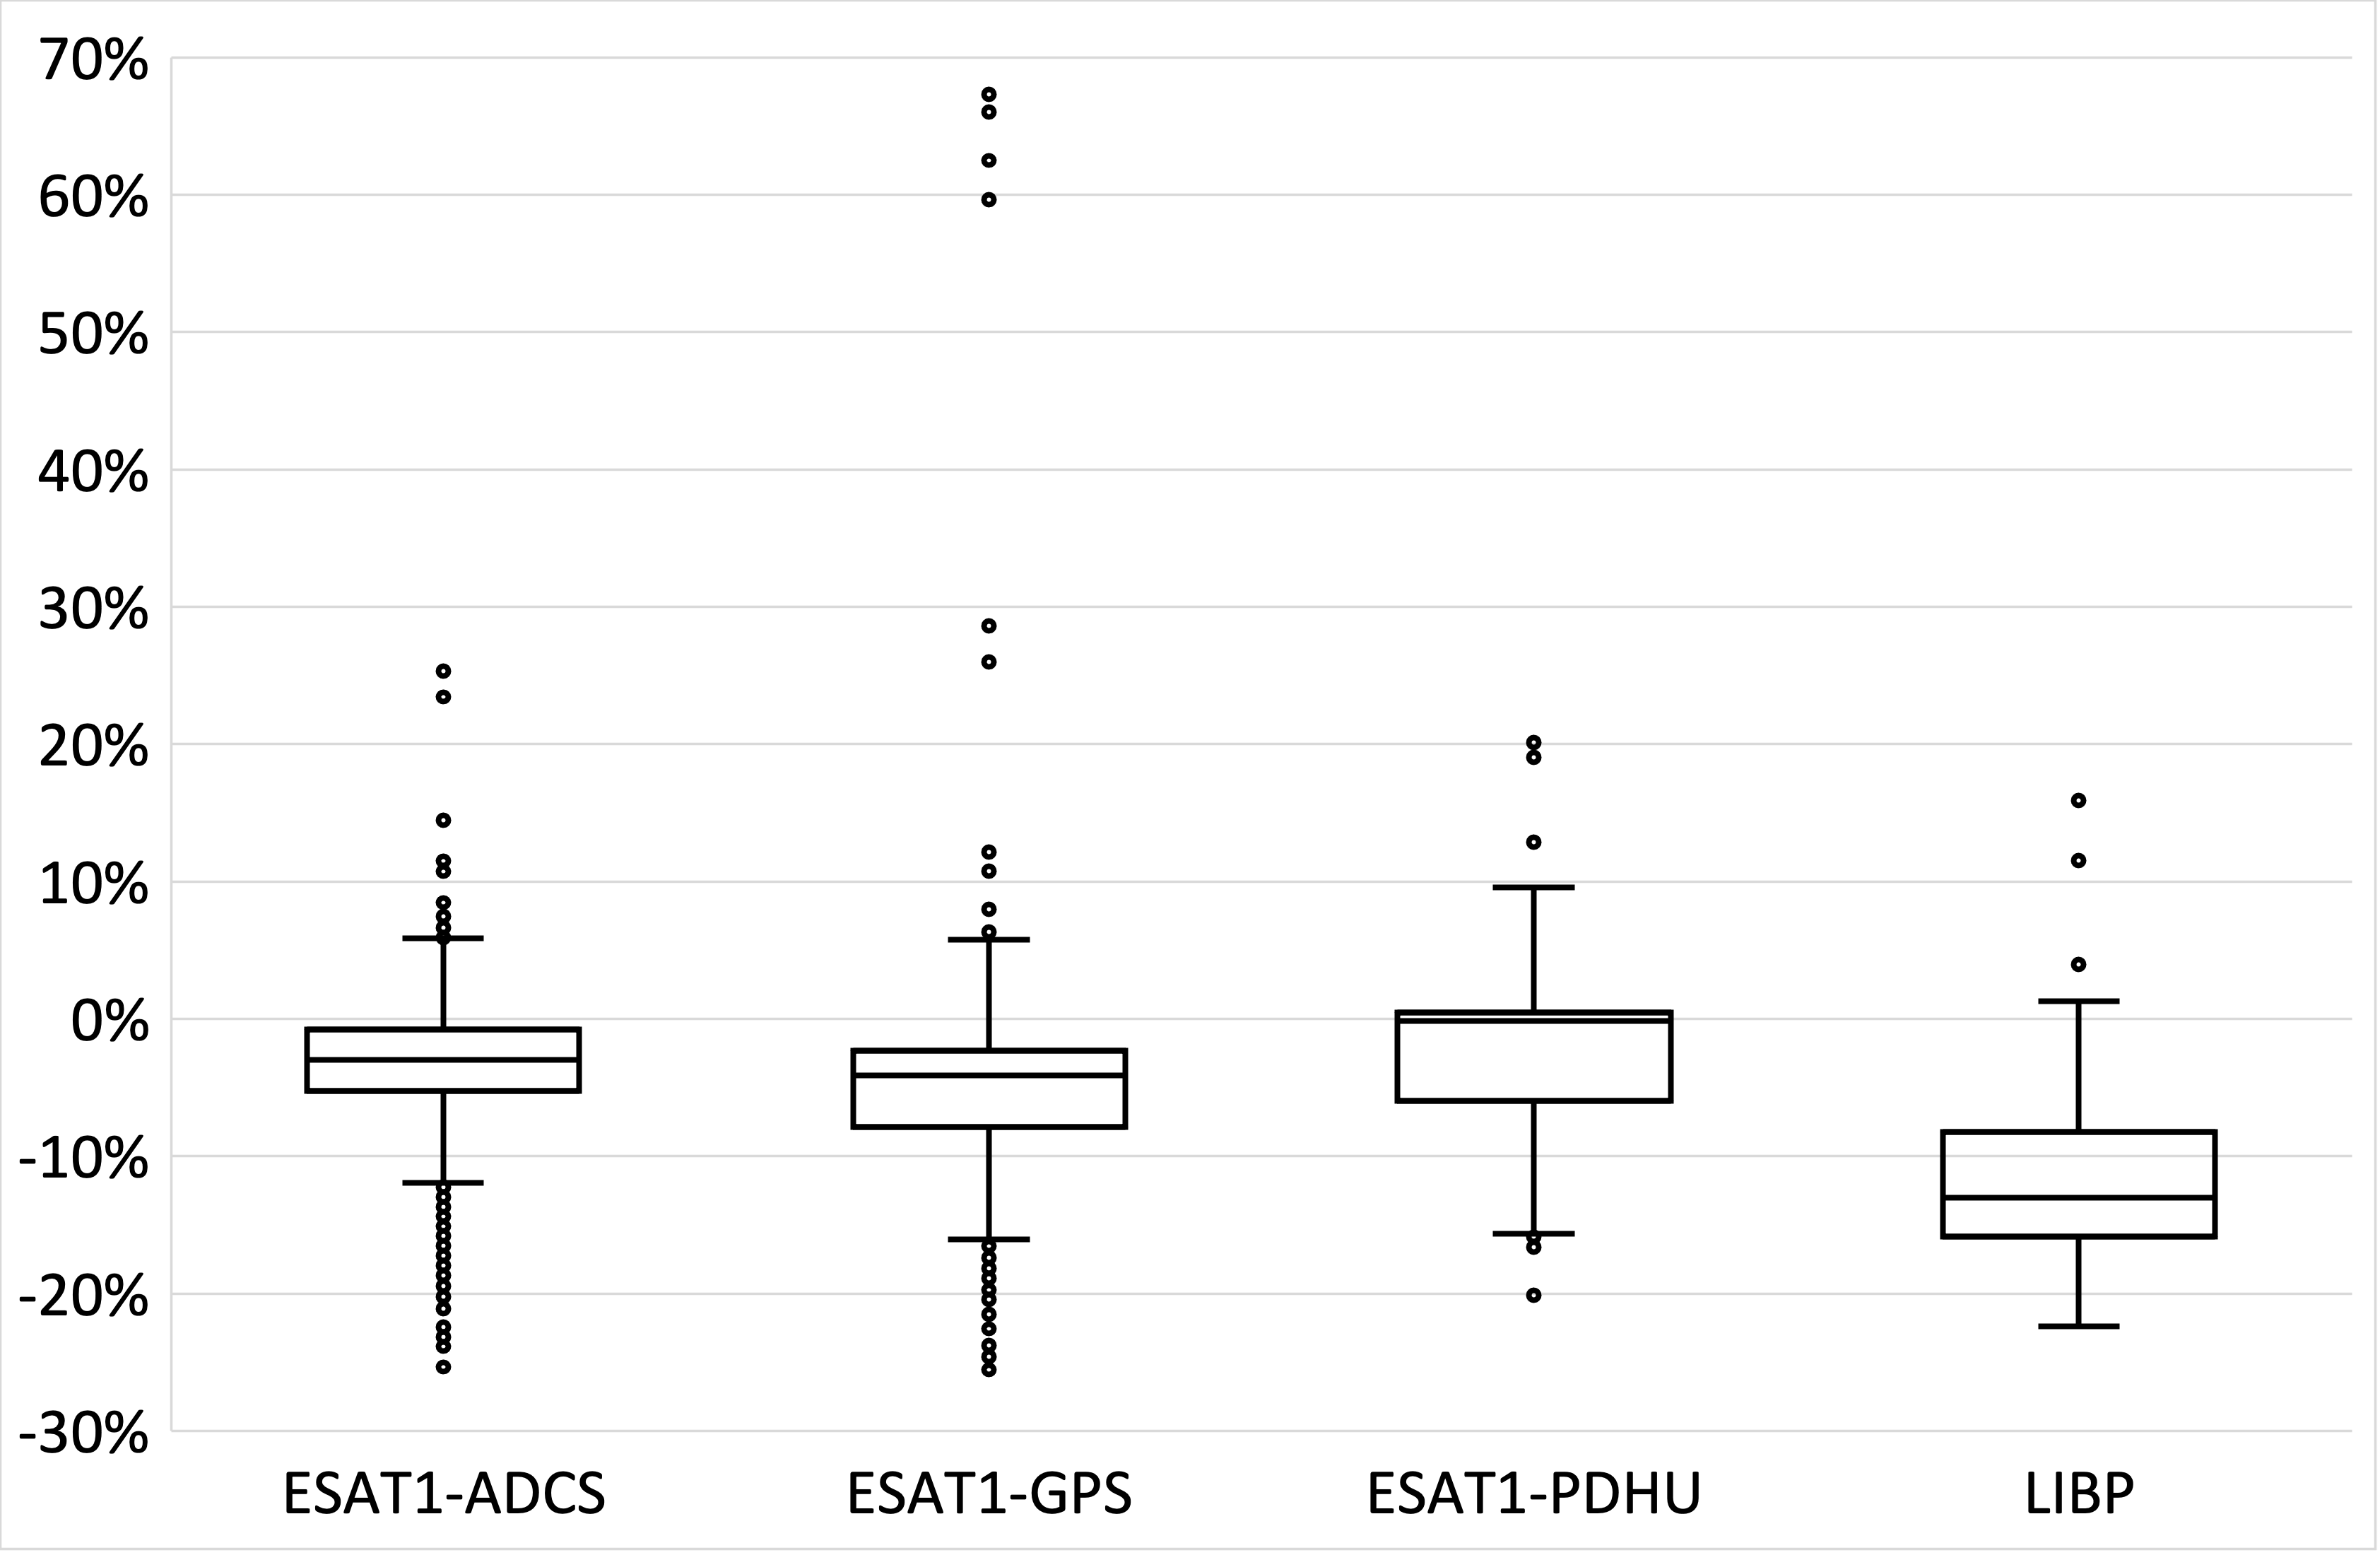
\includegraphics[width=0.8\columnwidth]{DDMA/images/overhead}
%        \caption{\APPR execution overhead per mutant.}
%        \label{fig:appr:overhead}
%    \end{figure}


% \subsection{RQ5 - Relation between data-driven and code-driven mutation analysis}

% \subsubsection*{Design and measurements}

% RQ5 aims to evaluate if data-driven mutation analysis is an alternative to code-driven analysis for a same execution cost (i.e., same number of mutants).
% Particularly, we aim to determine if data-driven mutation analysis subsumes the code-driven one when a same number of mutants is considered. Data-driven mutation analysis subsumes code-driven mutation analysis if
% the set of test cases that achieve maximal mutation analysis results for data-driven mutation analysis achieves the maximal mutation analysis results also for code-driven mutation analysis.
% %every test case that kills a data-driven mutant is guaranteed to also kill a code-driven mutant.

% Since in our context it is not possible to automatically generate 100\% mutation score we assume that the mutation analysis results achieved by the existing test suites are the maximal achievable.

% In practice, we perform an experiment in which we remove all the test cases that kill data-driven mutants and evaluate the effect on the mutation score for the code-driven mutants (hereafter, code-driven mutation score).
% More specifically, (1) we randomly select $N$ code-driven mutants (being $N$ equal to the number of data-driven mutation operations for a specific subject) generated with an extended version of SRCIRor~\cite{hariri2018srciror} from a set of source files targeting the system or sub-system under analysis.
% (2) We execute the code-driven mutants against the test suite without the test cases killing all data-driven mutants,
% and (3) we compute the mutation score of such set.
% If data-driven mutation analysis subsumes code-driven mutation analysis the
% code-driven mutation score
% shall be close to zero.
% To account for randomness we repeat the experiment 5 times.

% Similarly, we study if code-driven subsumes data-driven mutation analysis by removing all the test cases that kill code-driven mutants and evaluate the effect on the data-driven mutation analysis result. %mutation score for the data-driven mutants.

% On one hand, the nature of code-driven mutation analysis causes the technique to generate a large number of mutants (e.g., hundreds of thousands of mutants~\cite{papadakis2019mutation,zhang2013operator} can be generated for a 70K LoC system), scenario that can be worsened when considering the complexity and size of CPS software, combined with its high test execution cost.
% On the other hand, data-driven mutation analysis simulates high level faults on interoperability of integrated components, which generates by its nature, a smaller set of mutants (i.e., between 20 and 120 mutants in our subjects).
% Consequently, a reasonable idea would be to consider data-driven mutation analysis rather than code-driven mutation analysis, because of its lower cost.

% To verify the subsumption relation,

% for each data-driven mutant, we measure the overall number of code-driven mutants non detected when removing the test set killing such data-driven mutant.
% If the resulting distribution of non detected code-driven mutant has an average/median close ($\pm 5\%$) to the total number of originally killed code-driven mutants, means that code-driven mutation was subsumed by data-driven mutation analysis.


% we measure the overall number of code-driven mutants not detected when removing a test case killing a data-driven mutant. If the number is high, it means that data-driven mutation enable to detect more limitations than code-driven mutation.


% To do so, for every subject, and for each data-driven mutant, we remove the test cases that kill the mutant and measure how many code-driven mutants are no longer detected. Then, in a similar way, for each code-driven mutant, we remove the test cases that kill the mutant and measure how many data-driven mutants are no longer detected.
% When comparing data-driven and code-driven approaches for a specific subject, we consider the same number of mutants (e.g., for the \ADCS subjects we generate 119 data-driven mutants, and 119 code-driven mutants).

% For the assessment of code-driven mutants on our subjects %we use MASS~\cite{}
% we performed the following steps: (1) we used a extended version of SRCIRor~\cite{hariri2018srciror} for the generation of mutants based on the test suite's code coverage, (2) we disregarded equivalent and redundant mutants based on trivial compiler optimizations~\cite{kintis2017detecting}, (3) we randomly sampled $N$ mutants from the whole set and (4) we executed the test suite against the sampled mutants.

% We study the distribution of the code-driven mutants not detected when removing a test case killing a data-driven mutant.
% We also study the distribution of the data-driven mutants not detected when removing a test case that kills a code-driven mutant.
% To analyze the distributions we use a t-test that enables the comparison of two distributions.
% If both distributions have similar means, it indicates that each technique kill a set of mutants that is different from the other approach. In the case that both distribution have different means, it means that one technique kills a set of mutant that includes the set of killed mutants of the other technique.




% \subsubsection*{Results}
% \TODO{TBD}



\subsection{Threats to validity}
\label{sec:threats:damat}

%To ensure the same conditions to all mutant executions, we run each test suite in a clean instance of a virtualized environment.}

\emph{Generalizability}. We have selected industrial software systems of diverse size, tested with different types of test suites. They are developed according to space safety standards and are thus  representative of software system software adhering to safety regulations.
\REVOCT{C-P-16}{We expect our results to generalize for systems with architectures similar to \SAIL  and libParam, which have a client/server architecture, which is standard practice. For \SAIL the ADCS, GPS, and PDHU act as distinct servers and the control software is the client that requests information; libParam has a standard client/server structure.}
Also, \ESAIL is larger than any other industrial system considered in the mutation analysis literature to date~\cite{Ramler2017,delgado2018evaluation,Baker2013,denisov2018mull}.

{\emph{Internal}. To minimize implementation errors, we have extensively tested our toolset.}

{\emph{Construct}. The indicators selected for cost estimation (configured operators and LoC) are directly linked to the activities of the end-user and are thus appropriate. We leave empirical studies with human subjects to future work. To discuss overhead, we rely on test execution time, which may be affected by other factors than mutation overhead (e.g., the system behaves differently with mutated data). Dedicated benchmarks might be an alternative.}

{\emph{Conclusion}. To ensure reliability, for RQ1 and RQ2, we confirmed our findings with engineers.}

%However, we realize that the procedure we followed for the selection of pairs of mutants, only showed additional ways to improve and augment a test suite.
%For example, for the \ADCS subject, the procedure showed that two mutants from the same fault model (i.e., SunSensorTM), but targeting different data items, data item 0 and 28 respectively, are failing in the same way. This is not a sign of mutant redundancy, but an evidence that test suite should distinguish the two mutants independently, through two different test cases.
%
%This is in line with related work~\cite{}, showing that test suites should be augmented with additional test cases to make a single mutant fail.


% \subsection{RQ6 - Mutation operation coverage}

% % \subsubsection*{Design and measurements}

% % Given that CPSs are usually constrained by very %strict time limits
% % hard real-time requirements, it may make sense to limit the number of times a mutation probe is activated, to avoid interfering with real-time tasks.

% % Depending on how often test checks (e.g., test assertions) are performed, it may make sense to reduce the number of times a mutation is performed. For example, short test cases (e.g., unit test cases) often verify every value under test, so even mutating a portion of them might lead to a test fail.
% % Surely, by reducing the number of times a mutation is performed, we might decrease the chances of a mutant being killed.

% Because of the complexity and size of CPSs, combined with its high test execution cost, we are interested in limiting the number of times a mutation probe is activated.
% To this end, we aim to study how mutation analysis results vary when changing the proportion of data item instances to mutate.

% % Our goal is to determine the quality of CPS test suites in terms of how often test checks are performed during test suite execution. For instance, a high quality test suite shall detect every mutated data, so in the case that a mutation is applied once, there should be a failing test case.

% Our goal is to provide guidelines for mutants sampling (i.e., the probability of executing a mutant) to determine if there exists a threshold for the sampling rate that makes it likely to detect all the limitations of a test suite.

% To do so, for each subject, we consider the three cases described in Section~\ref{sec:mutantsExecution}:

% \begin{enumerate}
%     \item The mutation is applied only once,
%     for every test case, on the first data item instance processed by the mutation probe.
%     %the mutation occurs the first time the mutant is executed.
%     \item The mutation is applied on every data item instance processed by the mutation probe.
%     \item The mutation is applied with a probability $p$, ranging from 10\% to 90\%, in steps of 10\%.
% \end{enumerate}


% %For each probability $p$ of setup (2),
% To account for randomness, we repeat the experiment 5 times.
% %, i.e., we compute the mutation score 5 times, based on 5 executions of all mutants against the subject test suite.

% %We discuss the setup that provides the closest mutation score with respect to the mutation score obtained when mutating all the times.

% We identify the differences between the mutation analysis results obtained across the configurations specified above and assess the significance of such differences.

% \subsubsection*{Results}
% \TODO{TBD}

% \subsubsection*{Results}
% \TODO{TBD}
